\section{Problem}
% TODO What is the problem and why do we care

\subsection{Background}

\begin{frame}
\begin{itemize}
  \item Many interesting problems require processing graph data for real world applications \linebreak
  \begin{itemize}
  \item Data Mining
  \item Page Rank
  \item Social Networking
  \item Online Machine Learning
  \item Business Intelligence
  \item Analytics
  \end{itemize}	
\end{itemize}	
\end{frame}

\begin{frame}
\begin{itemize}
  \item The scale of these graph, in some case contains billions of vertices, trillions of edges - poses a challenge to efficient processing
  \linebreak
  \item Numerous frameworks have been developed to process these graphs efficiently (e.g. Pregel, GraphX, Giraph, Mizan, GraphLab, GPS, etc)
\end{itemize}	
\end{frame}

\begin{frame}
	 \begin{figure}
			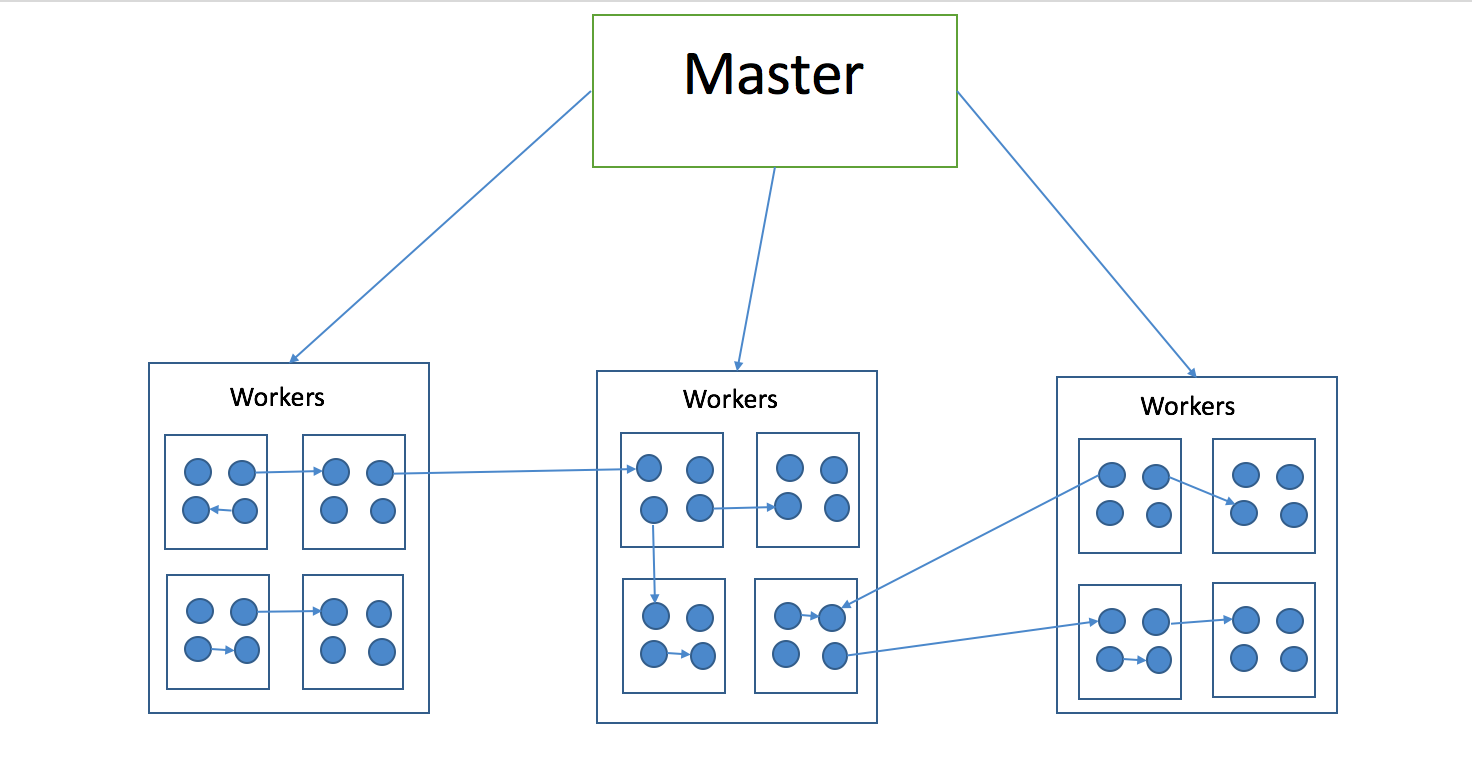
\includegraphics[width=0.8\linewidth]{figures/execution1.png}
	\caption{Execution model of Pregel}
	\end{figure}
 \end{frame}	
	

\begin{frame}
\begin{itemize}
  \item Some graph algorithms requires a combination of vertex-centric (parallel) and global (sequential) computations
  	\begin{itemize}
	 \item An example could be k-means-like graph clustering algorithm
	 \end{itemize}
  \item This type of algorithm requires a means of graph mutation operations
   \item These graph processing frameworks provide the means of graph mutation
     	\begin{itemize}
		\item e.g.: Pregel, Giraph, Mizan, GPS, Graph Lab (supports partial mutation)
			 \end{itemize}
\end{itemize}	
\end{frame}


\begin{frame}
  	\begin{itemize}
		\item However, topology mutation operations performed concurrently at different vertices can conflict with each other
		 \item All these graph processing frameworks resolve the mutation conflicts by using:
  	  		\begin{itemize}
				\item Partial ordering : edge remove $\rightarrow$ vertex remove $\rightarrow$ vertex add $\rightarrow$ edge add
			\item User defined handlers
		\end{itemize}
		\item Conflicts not solvable by the reordering are expected to be solved by the programmer
	  \end{itemize}
\end{frame}

\section{Examples}
\subsection{Problem Example}
\begin{frame}[fragile]
\begin{lstlisting}[
    language=Java]
  public interface Computation<I, V, E, M>{
    void compute(Vertex<I,V,E> vertex, Iterable<M> messages);
    //Must be defined by user to do computation on a single Vertex.
	
    void 	addEdgeRequest(I sourceVertexId, Edge<I,E> edge);
    void 	addVertexRequest(I id, V value);
    void 	removeEdgesRequest(I sourceVertexId, I targetVertexId);
    void 	removeVertexRequest(I vertexId);
    long 	getSuperstep();
    long 	getTotalNumEdges();
    long 	getTotalNumVertices();
    void 	postSuperstep();
    void 	preSuperstep();
    void 	sendMessage(I id, M message);
  }
\end{lstlisting}
Essential operations of a \textit{Computation} in Giraph
\let\thefootnote\relax\footnotetext{\tiny[giraph.apache.org/apidocs/]}
\end{frame}

\begin{frame}[fragile]
\begin{lstlisting}[
    language=Java]
  Public class SimpleMutateGraphComputation extends BasicComputation<
    LongWritable, DoubleWritable, FloatWritable, DoubleWritable> {

    public void compute(Vertex<LongWritable, DoubleWritable, FloatWritable>
      vertex, Iterable<DoubleWritable> messages){ 
      if (getSuperstep() == 0) {
      	addVertexRequest(getVertexCount(), new
      	DoubleWritable(vertex.getValue()));
      } else if (getSuperstep() == 1) {
        vertex.voteToHalt();
    } 
  }
\end{lstlisting}
Example of a program that mutates a graph
\end{frame}

\subsection{Problem Context}
\begin{frame}
There are two kinds of conflicts:
\linebreak
\begin{itemize}
\item Conflicts such as the ones in the previous example still yields a well-formed graph after mutations, however the resulting graph is non deterministic
\linebreak
\item Another possibility for mutations is to produce an erroneous graph. e.g. one vertex adding an edge, and one vertex removing the vertex of the edge being added, resulting in a dangling edge
\end{itemize} 
\end{frame}

\begin{frame}
\begin{itemize}
\item The first type of conflict still produces a valid output, but may not be correct according the requirement of the program
\linebreak
\item The second type of conflict can happen because of the programmer's unawareness of the reordering, or algorithmic errors
\end{itemize} 
\end{frame}

\subsection{Problem Statement}
\begin{frame}
Our focus is to further solve these conflicts in 2 ways:
	\linebreak
	\\ 1. Analysis to identify the conflicts
	\linebreak
	\\ 2. Propose an abstraction for graph mutation that can avoid having nondeterministic mutations from happening
\end{frame}
